% --------------------------------------------------------------
% This is all preamble stuff that you don't have to worry about.
% Head down to where it says "Start here"
% --------------------------------------------------------------
 
\documentclass[12pt]{article}
 
\usepackage[margin=1in]{geometry} 
\usepackage{amsmath,amsthm,amssymb}
 \usepackage{graphicx, color}
\newcommand{\N}{\mathbb{N}}
\newcommand{\Z}{\mathbb{Z}}
 
\newenvironment{theorem}[2][Theorem]{\begin{trivlist}
\item[\hskip \labelsep {\bfseries #1}\hskip \labelsep {\bfseries #2.}]}{\end{trivlist}}
\newenvironment{lemma}[2][Lemma]{\begin{trivlist}
\item[\hskip \labelsep {\bfseries #1}\hskip \labelsep {\bfseries #2.}]}{\end{trivlist}}
\newenvironment{exercise}[2][Exercise]{\begin{trivlist}
\item[\hskip \labelsep {\bfseries #1}\hskip \labelsep {\bfseries #2.}]}{\end{trivlist}}
\newenvironment{reflection}[2][Reflection]{\begin{trivlist}
\item[\hskip \labelsep {\bfseries #1}\hskip \labelsep {\bfseries #2.}]}{\end{trivlist}}
\newenvironment{proposition}[2][Proposition]{\begin{trivlist}
\item[\hskip \labelsep {\bfseries #1}\hskip \labelsep {\bfseries #2.}]}{\end{trivlist}}
\newenvironment{corollary}[2][Corollary]{\begin{trivlist}
\item[\hskip \labelsep {\bfseries #1}\hskip \labelsep {\bfseries #2.}]}{\end{trivlist}}
 
\begin{document}
 
% --------------------------------------------------------------
%                         Start here
% --------------------------------------------------------------
 
%\renewcommand{\qedsymbol}{\filledbox}
 
\title{Programming Assignment 1}%replace X with the appropriate number
\author{Sneha Reddy Aenugu, EE11B059\\ %replace with your name
} %if necessary, replace with your course title
 
\maketitle

\section{Linear Classifier}
 
\begin{itemize}
\item{The dataset is generated with the required constraints and is attached in the zip file as \emph{DS1}}
\item{Figure 1 gives the estimated coefficients of the regression model.
\begin{figure}
	\centering
		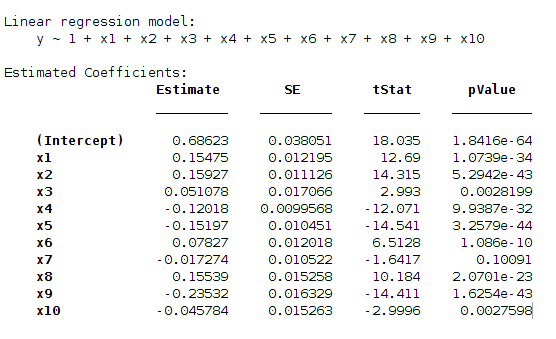
\includegraphics[scale = 0.7]{/home/sneha/Acads/9thsem/ML/P1/Pics/pic1.png}
	\caption{Estimated coefficients of the regression model}
	
\end{figure}}

Accuracy of the regression classifier = 89.75\%
Root Mean Squared Error = 0.311

\item{ Table 1 gives accuracy of KNN classifiers for different values of k.
\begin{table}
\centering
		\begin{tabular}{|l | r|}
			\hline
			\textbf{k} & \textbf{Accuracy} \\ \hline
			 1 & 74 \\ \hline
			2 & 74\\ \hline
			3 & 82.25  \\ \hline
			 4  & 81.25\\ \hline
			5 & 83.75 \\ \hline
			6 & 82.75 \\ \hline
			7 & 82.5 \\ \hline
			8 & 82.25 \\ \hline
			9 & 83.75 \\ \hline
			10 & 83.5 \\ \hline
			11& 83 \\ \hline
			12& 82.25 \\ \hline
			13& 83 \\ \hline
			
			
		\end{tabular}
	\caption{Accuracy in knn-classifier}

\end{table}

KNN is not better than the regression.There are few values of k where accuracy goes up slightly as shown in Table 1}

\end{itemize}

\section{Linear Regression}
\begin{itemize}
\item{ Among all the features there are 22 features which have 1675 features missing out of 1994 features. So these features were discarded because of the uncertainty in the readings.}

\item{ The coefficients learned are a vector of 101 features and the model is given in the zip file submitted. The Root Mean Squared Error for the problem is 0.132.}


\end{itemize}
\section{Feature Selection}
\begin{itemize}
\item{Figure 2 shows the 3D plot of the dataset. The figure shows the data is seperable in one dimension. PCA is performed on the dataset and a single feature is extracted. The extracted features are then fitted with the indicator variables given by the labels using linear regression. The linear model is then used to predict the classes of the test dataset. Figure 2 plots the data points with their labels. The decision boundary used for classification is also included. Figure 3 plots the predicted value of the datapoints with the threshold line. \\


\begin{equation}
Confusion\ Matrix = \begin{bmatrix} 150 & 50 &\\ 42 &158 \end{bmatrix}
\end{equation}
Class 1:

\begin{equation}
Precision = \frac{150}{150+42} = 0.78
\end{equation}
\begin{equation}
Recall = \frac{150}{150+50} = 0.75
\end{equation}
\begin{equation}
f-measure = 2*\frac{Precision*Recall}{Precision + Recall} = 0.76
\end{equation}
Class 2:

\begin{equation}
Precision = \frac{158}{158+50} = 0.76
\end{equation}
\begin{equation}
Recall = \frac{158}{158+42} = 0.77
\end{equation}
\begin{equation}
f-measure = 2*\frac{Precision*Recall}{Precision + Recall} = 0.76
\end{equation}


\begin{figure}


	\centering
		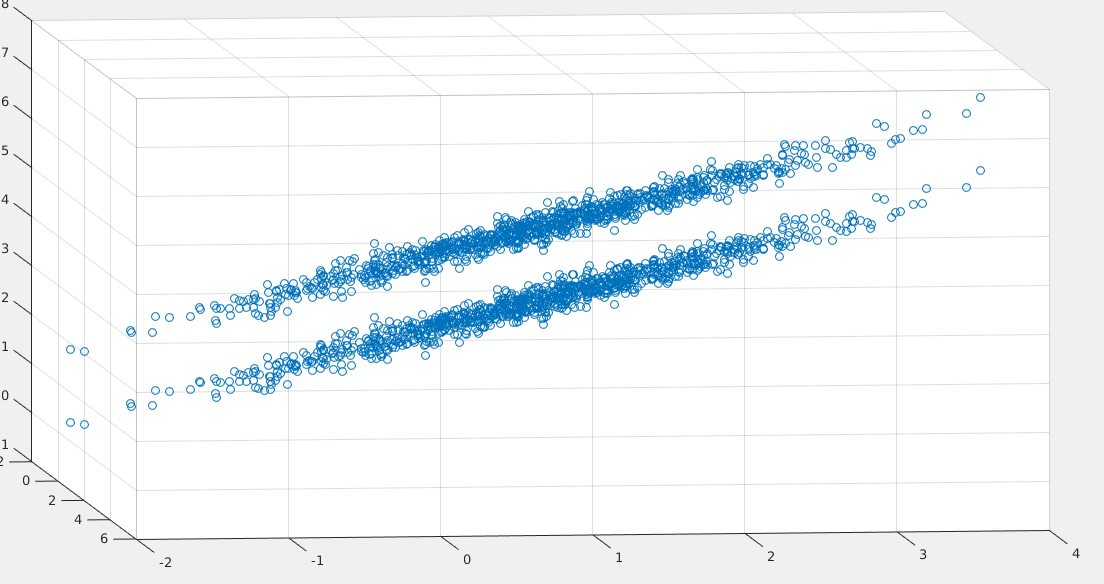
\includegraphics[scale = 0.3]{/home/sneha/Acads/9thsem/ML/P1/Pics/pic2.png}
	\caption{3D plot of the dataset}
	
\end{figure}


\begin{figure}
	\centering
		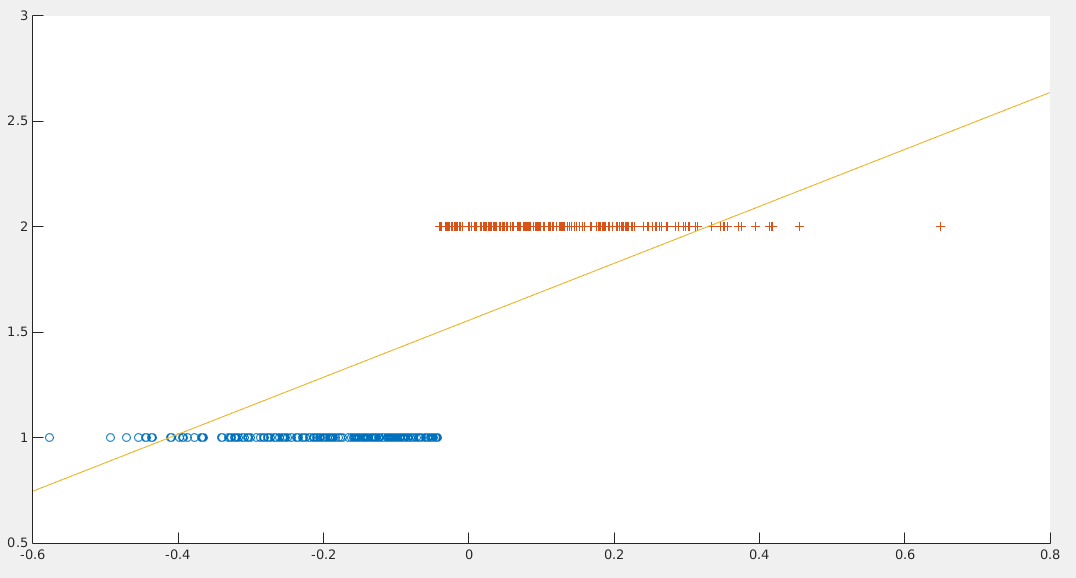
\includegraphics[scale = 0.3]{/home/sneha/Acads/9thsem/ML/P1/Pics/pic3.png}
	\caption{Projected feature space with the decision boundary}
	
\end{figure}

\begin{figure}
	\centering
		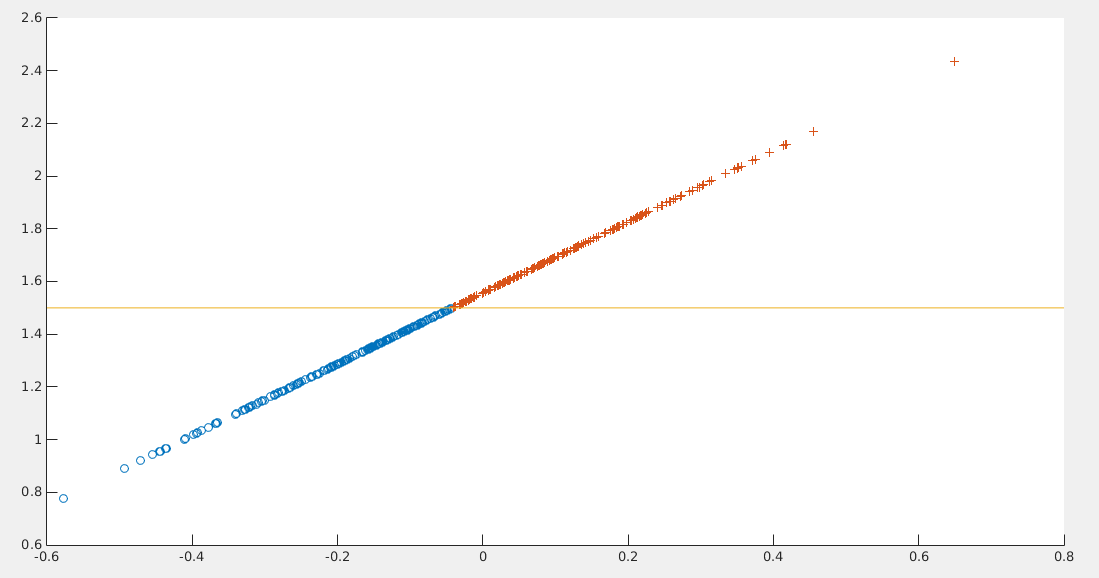
\includegraphics[scale = 0.3]{/home/sneha/Acads/9thsem/ML/P1/Pics/pic4.png}
	\caption{Projected feature space with the threshold}
	
\end{figure}

}

\item{Performing LDA to the same data set shows a remarkable increase in the efficiency of classification. The per-class precision and recall of each class equal to 1
\begin{equation}
Confusion\ Matrix = \begin{bmatrix}200  & 0 &\\ 0 &200 \end{bmatrix}
\end{equation}
Class 1:

\begin{equation}
Precision = 1
\end{equation}
\begin{equation}
Recall = 1
\end{equation}
\begin{equation}
f-measure = 1
\end{equation}
Class 2:

\begin{equation}
Precision = 1
\end{equation}
\begin{equation}
Recall = 1
\end{equation}
\begin{equation}
f-measure = 1
\end{equation}
\begin{figure}
	\centering
		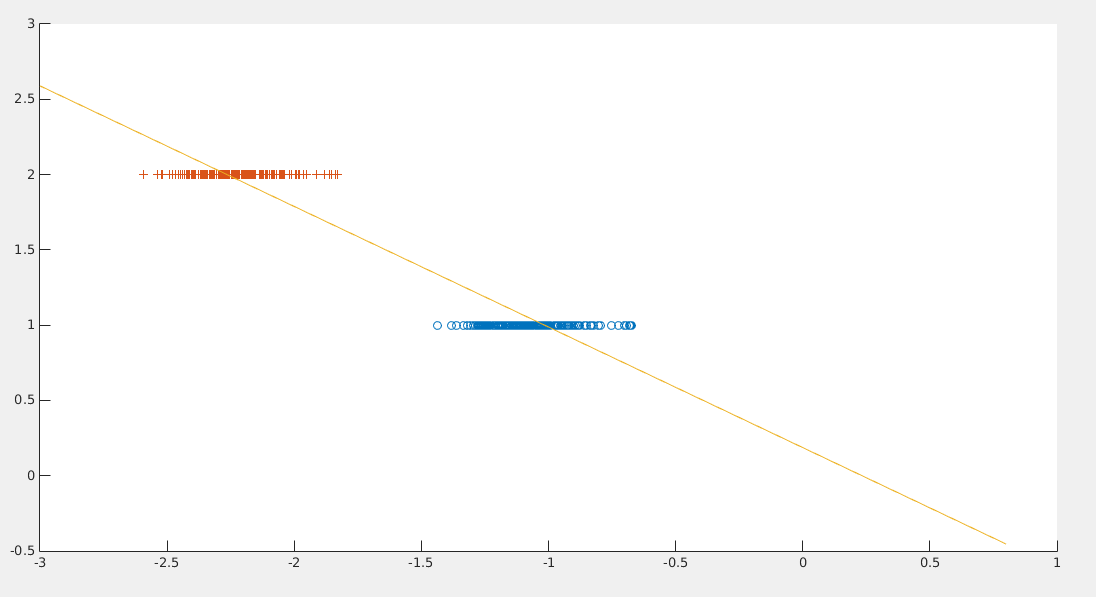
\includegraphics[scale = 0.3]{/home/sneha/Acads/9thsem/ML/P1/Pics/pic5.png}
	\caption{Projected feature space with the decision boundary}
	
\end{figure}

\begin{figure}
	\centering
		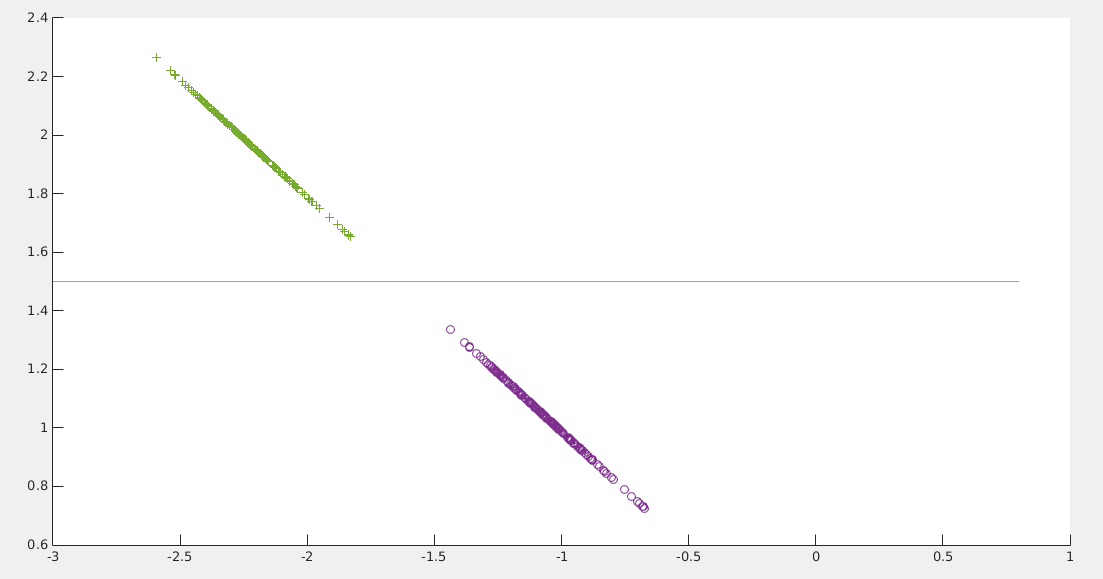
\includegraphics[scale = 0.3]{/home/sneha/Acads/9thsem/ML/P1/Pics/pic6.png}
	\caption{Projected feature space with the threshold}
	
\end{figure}

}

\end{itemize}


\section{Support Vector Machines}
A 96 dimensional feature vector is employed for the classification of the images into the 4 categories forest, insidecity, coast, mountain. Four kernel functions are used for the purpose of classification and the kernal parameters and accuracy are tabulated in Table 2.\\
\begin{table}

\begin{center}
		\begin{tabular}{|c |c | c | c | c |}
			\hline
			\textbf{Kernelfunction}  & \textbf{gamma} & \textbf{coef0} & \textbf{cost} & \textbf{Accuracy} \\ \hline
			 Linear & 0.01 & 0 & 20 & 65.06 \\ \hline
			Polynomial (degree 2) & 0.1 & 10 & 1 & 65.06\\ \hline
			Radial Basis Function & 0.1 & 0 & 1 & 68.67   \\ \hline
			Sigmoid & 0.01 & -1 & 1 & 66.26 \\ \hline
			
			
			
		\end{tabular}
\end{center}
\caption{Accuracy in knn-classifier}
\end{table}

The training models generated by the each kernel function are provided in the zip file named as model0, model1, model2, model3 respectively for Linear, Polynomial, Radial Basis Function and Sigmoid functions. 	


\section{Bayesian Parameter Estimation}
 \begin{itemize}
 
\item{\textbf{Multinomial likelihood:}The 5 confusion matrices obtained through cross validation are given below.
\begin{equation}
Confusion\ Matrix1 = \begin{bmatrix}119  & 2 &\\ 5 &95 \end{bmatrix}
\end{equation}
\begin{equation}
Confusion\ Matrix2 = \begin{bmatrix}184  & 1 &\\ 2 &144 \end{bmatrix}
\end{equation}
\begin{equation}
Confusion\ Matrix3 = \begin{bmatrix}243  & 2 &\\ 5 &191 \end{bmatrix}
\end{equation}
\begin{equation}
Confusion\ Matrix4 = \begin{bmatrix}303  & 3 &\\ 6 &238 \end{bmatrix}
\end{equation}
\begin{equation}
Confusion\ Matrix5 = \begin{bmatrix}367  & 2 &\\ 4 &287 \end{bmatrix}
\end{equation}

\textbf{Average per class Precision}

Legit mails = 99.09\% \\
Spam mails  = 97.44\%

\textbf{Average per class Recall}

Legit mails = 97.97\% \\
Spam mails  = 98.85\%

}



\item{\textbf{Bernoulli likelihood:} The 5 confusion matrices obtained through cross validated are given below.
\begin{equation}
Confusion\ Matrix1 = \begin{bmatrix}123  & 1 &\\ 24 &73 \end{bmatrix}
\end{equation}
\begin{equation}
Confusion\ Matrix2 = \begin{bmatrix}186  & 0 &\\ 12 &133 \end{bmatrix}
\end{equation}
\begin{equation}
Confusion\ Matrix3 = \begin{bmatrix}248  & 0 &\\ 12 &181 \end{bmatrix}
\end{equation}
\begin{equation}
Confusion\ Matrix4 = \begin{bmatrix}309  & 0 &\\ 17 &224 \end{bmatrix}
\end{equation}
\begin{equation}
Confusion\ Matrix5 = \begin{bmatrix}369  & 2 &\\ 17 &272 \end{bmatrix}
\end{equation}

\textbf{Average per class Precision}

Legit mails = 92.68\% \\
Spam mails  = 99.58\%   

\textbf{Average per class Recall}

Legit mails = 99.73\%\\
Spam mails  = 89.57\%

}

\item{ \textbf{Beta Prior :}The optimum value of $ \alpha $ and $ \beta $ which give the best value of $ Precision * Recall $ is $ \alpha = 9$ and $ \beta = 2 $. \\
The P-R curve for the following in given in the figure
\begin{figure}


	\centering
		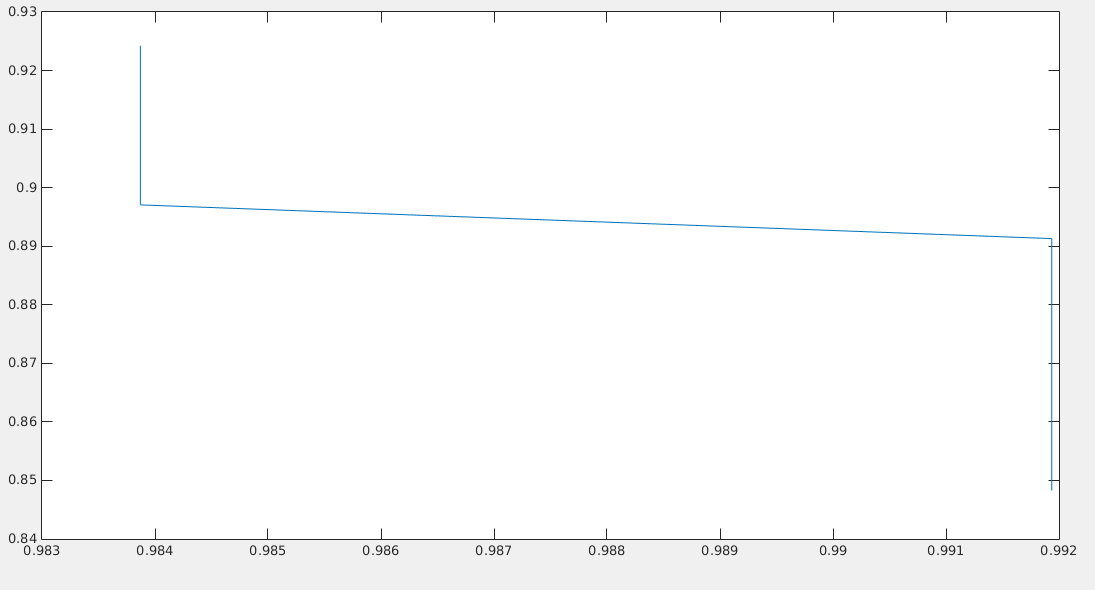
\includegraphics[scale = 0.3]{/home/sneha/Acads/9thsem/ML/P1/Pics/pic7.png}
	\caption{P-R curve for beta prior}
	
\end{figure}
}
 \end{itemize}


% --------------------------------------------------------------
%     You don't have to mess with anything below this line.
% --------------------------------------------------------------
 
\end{document}